% Provenance (never printed): cycle 3 / 6e "La planete Terre" (rocks and
% minerals; the three rock families; recognising common rocks); see
% sources/book1/PROVENANCE.md. Book 1, grade 6, chapter 3.
% Vocabulary guard: "magma" not before g7.2 (here "molten rock");
% "sediment" not before g7.4 (here "grains of sand and mud").
\chapter{Roches et minéraux}\label{ch:g6:rocks-and-minerals}

Sam se penche sur le plan de travail de la cuisine avec une loupe. La
pierre polie, qui paraît grise de loin, devient une foule de petites
taches~: des roses, des blanches, des grises et vitreuses, et de minuscules
noires qui brillent quand la lumière les accroche. Chaque tache a des faces
plates et brillantes, et les taches s'emboîtent comme les pièces d'un
puzzle. Que sont-elles~?

\begin{omfigure}
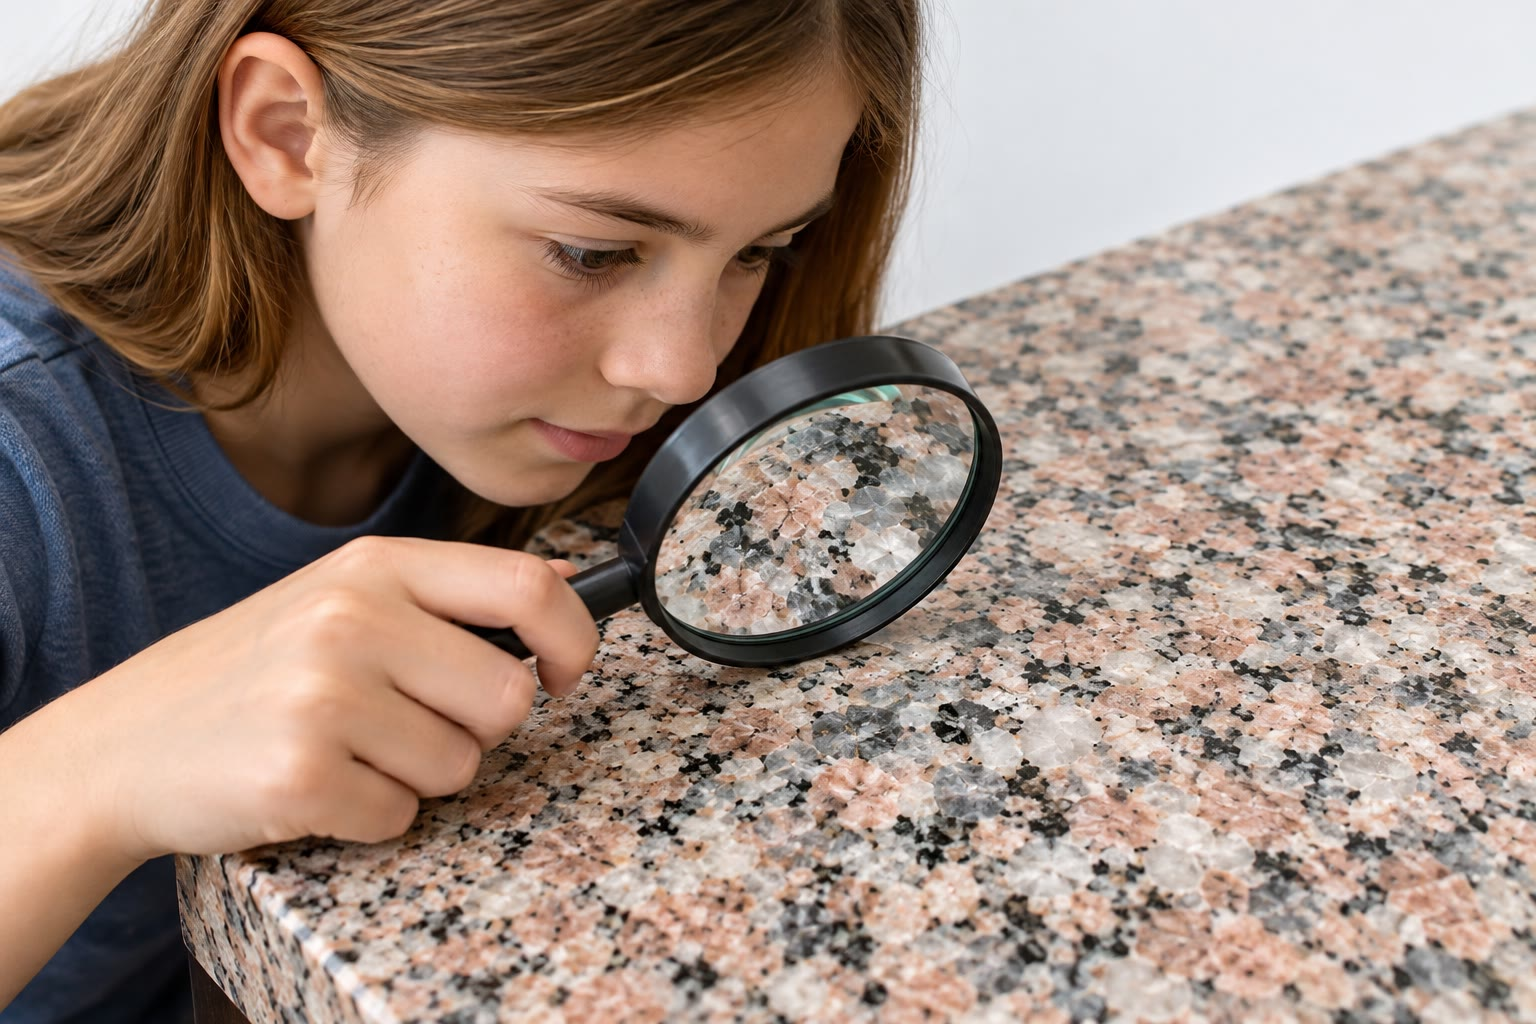
\includegraphics[width=0.6\linewidth]{images/book1/ai/g6-hand-lens-worktop.jpg}

{\small Un plan de travail en pierre tachetée, observé à la loupe.
(Illustration générée par IA.)}
\end{omfigure}

\begin{recall}
Les \omterm{def:g3:stones-pebbles-sand:rock}{roches} sont le matériau dur de la croûte terrestre~: on peut les briser
en cailloux, les \omterm{def:g1:landscapes-around-us:water}{rivières} les roulent en \omterm{def:g3:stones-pebbles-sand:pebble}{galets}, et elles peuvent être
réduites en \omterm{def:g3:stones-pebbles-sand:sand}{sable} (\cref{ch:g3:stones-pebbles-sand}). L'eau, la glace et
le vent usent les \omterm{def:g3:stones-pebbles-sand:rock}{roches} (\omterm{def:g5:water-shapes-the-land:weathering}{altération}), emportent les morceaux (\omterm{def:g5:water-shapes-the-land:erosion}{érosion}) et
les déposent plus loin (\omterm{def:g5:water-shapes-the-land:deposition}{dépôt}) (\cref{ch:g5:water-shapes-the-land}). Sur un
\omterm{def:g4:volcanoes-earthquakes-first-look:volcano}{volcan}, la \omterm{def:g3:stones-pebbles-sand:rock}{roche} fondue sort sous forme de \omterm{def:g4:volcanoes-earthquakes-first-look:eruption}{lave}
(\cref{ch:g4:volcanoes-earthquakes-first-look}).
\end{recall}

\section{Une roche est faite de minéraux}

Les petites taches du plan de travail sont des \omterm{def:g6:rocks-and-minerals:mineral}{minéraux}, et la pierre est un granite.

\begin{definition}[Minéral]\label{def:g6:rocks-and-minerals:mineral}
Un \emph{minéral}\index{mineral@minéral} est une substance solide
naturelle, qui n'est pas fabriquée par les êtres vivants, qui a toujours la
même composition et dont les atomes sont disposés de façon régulière. Une
\emph{\omterm{def:g3:stones-pebbles-sand:rock}{roche}} est faite d'un seul minéral ou, plus souvent, de plusieurs
minéraux assemblés.
% ledger: usgs:mineral-rock
\end{definition}

Le granite est fait surtout de trois \omterm{def:g6:rocks-and-minerals:mineral}{minéraux}~: le \emph{feldspath} (rose
ou blanc), le \emph{quartz} (gris et vitreux) et le \emph{mica} (noir ou
argenté, en fines paillettes brillantes). D'autres \omterm{def:g3:stones-pebbles-sand:rock}{roches} sont faites d'un
seul \omterm{def:g6:rocks-and-minerals:mineral}{minéral}~: le calcaire, par exemple, est fait presque uniquement de
calcite.
% ledger: nps:granite-minerals, usgs:mineral-rock

\begin{omfigure}
\begin{minipage}[c]{0.5\linewidth}\centering
\begin{tikzpicture}
  \begin{axis}[axis equal image, hide axis, width=\linewidth,
      xmin=0, xmax=6, ymin=0, ymax=4]
    \addplot[fill=orange!35!pink, draw=black!55, line width=0.4pt]
      table {figdata/out/grade-6-granite_mosaic-feldspar.dat};
    \addplot[fill=black!12, draw=black!55, line width=0.4pt]
      table {figdata/out/grade-6-granite_mosaic-quartz.dat};
    \addplot[fill=black!85, draw=black!55, line width=0.4pt]
      table {figdata/out/grade-6-granite_mosaic-mica.dat};
  \end{axis}
\end{tikzpicture}

{\small \tikz\fill[orange!35!pink, draw=black!55] (0,0) rectangle (0.25,0.18); feldspath\quad
\tikz\fill[black!12, draw=black!55] (0,0) rectangle (0.25,0.18); quartz\quad
\tikz\fill[black!85] (0,0) rectangle (0.25,0.18); mica}
\end{minipage}\hfill
\begin{minipage}[c]{0.46\linewidth}\centering
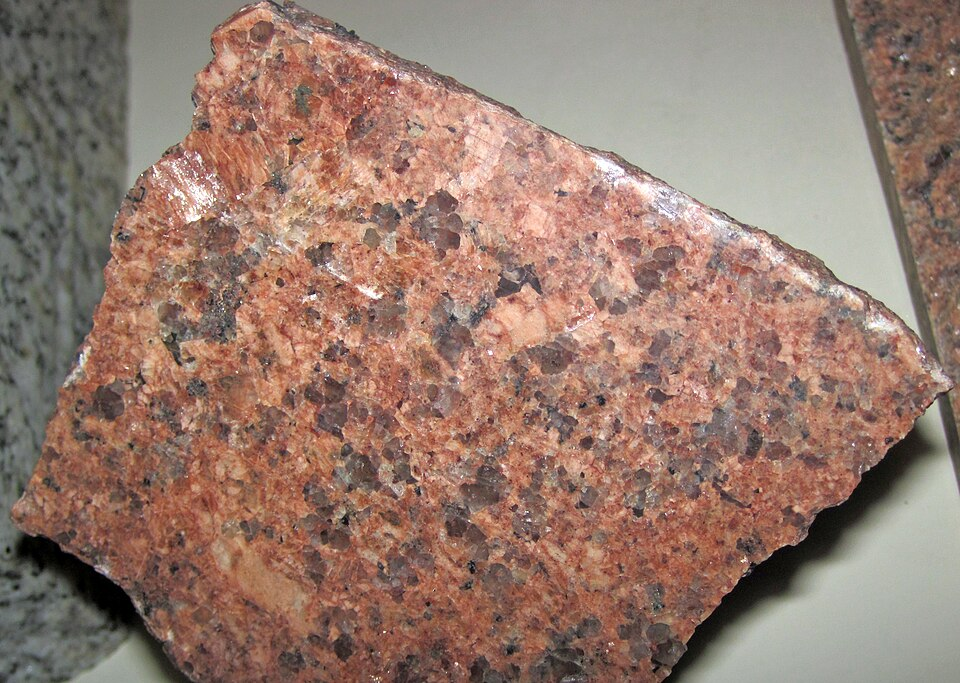
\includegraphics[width=\linewidth]{images/book1/g6-granite.jpg}
\end{minipage}

\smallskip
{\small À gauche~: le granite dessiné comme une mosaïque de grains, chaque
grain étant un \omterm{def:g6:rocks-and-minerals:mineral}{minéral} (agrandissement, pas à l'échelle). À droite~: un
vrai granite rose, de la taille d'une main environ.
(Photo~: James St.~John, CC BY 2.0, via Wikimedia Commons.)}
% ledger: nps:granite-minerals, commons:jsj-rocks (figdata/grade-6/granite_mosaic.py)
\end{omfigure}

\section{Les cristaux}

À la loupe, beaucoup de grains \omterm{def:g6:rocks-and-minerals:mineral}{minéraux} montrent des faces plates et
brillantes et des arêtes droites. Là où un \omterm{def:g6:rocks-and-minerals:mineral}{minéral} a eu la place de
grandir librement, dans un creux de la \omterm{def:g3:stones-pebbles-sand:rock}{roche}, il forme un cristal~: un
solide de forme régulière limité par des faces planes. Sa forme vient de
la disposition régulière de ses atomes, étudiée dans les livres de chimie.
Un cristal de quartz, par exemple, est une colonne à six faces qui se
termine en pointe~; un cristal de mica se débite en feuillets plus fins
que du papier.

\begin{omfigure}
\begin{minipage}[c]{0.2\linewidth}\centering
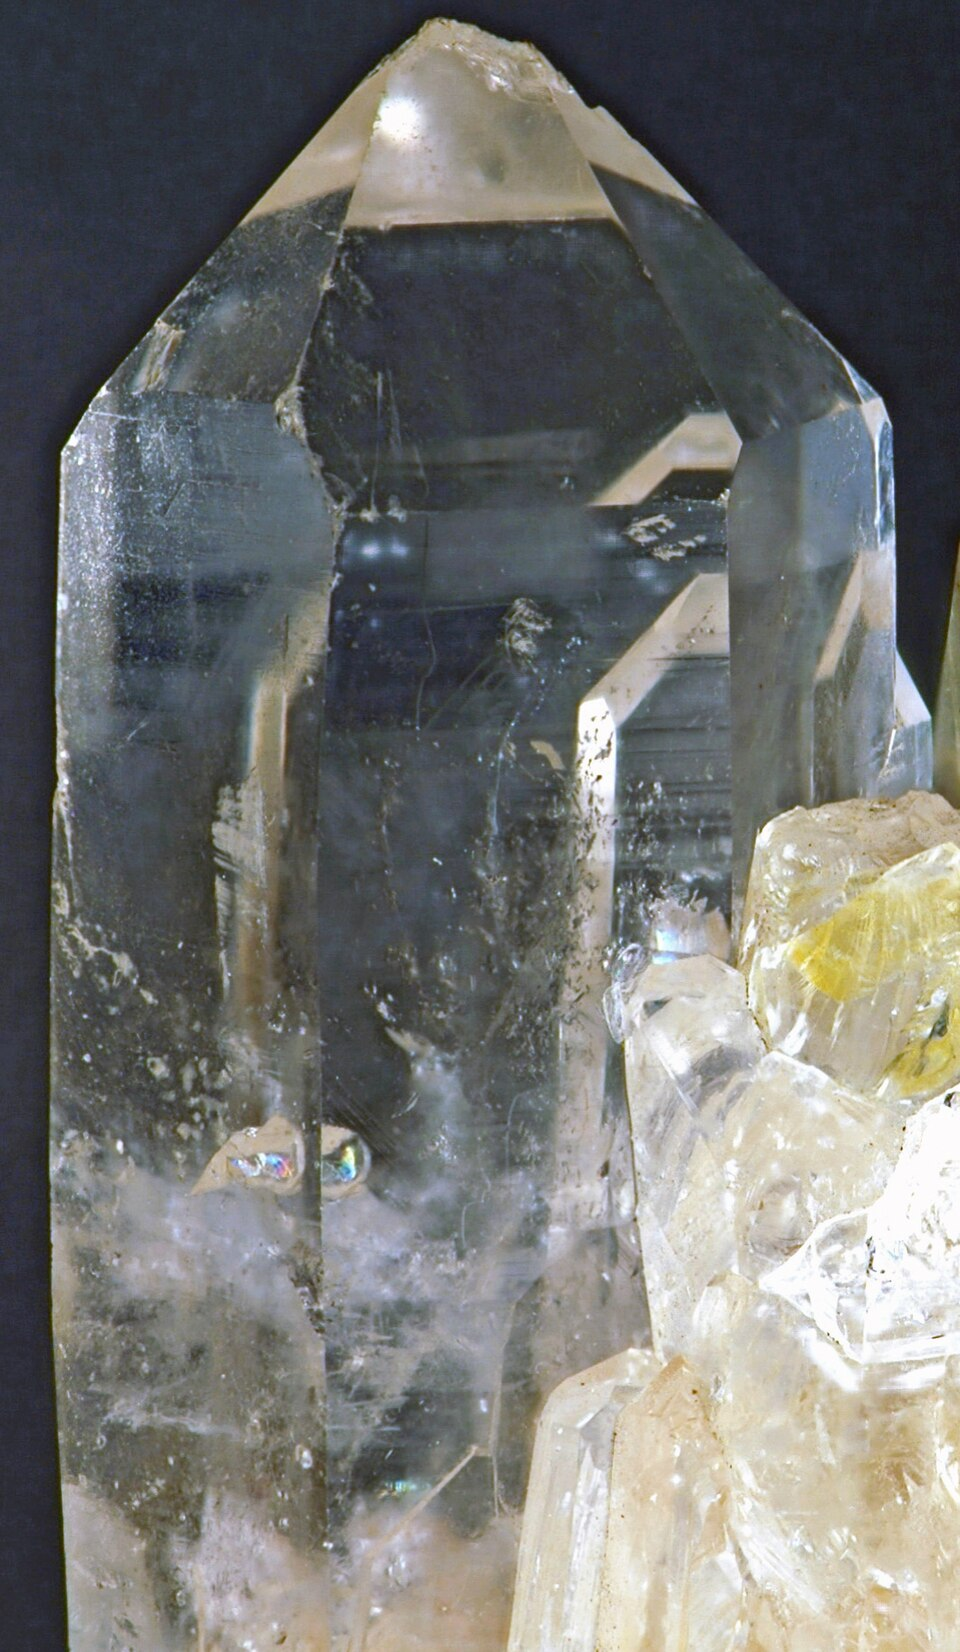
\includegraphics[height=4.2cm]{images/book1/g6-quartz.jpg}
\end{minipage}\hfill
\begin{minipage}[c]{0.44\linewidth}\centering
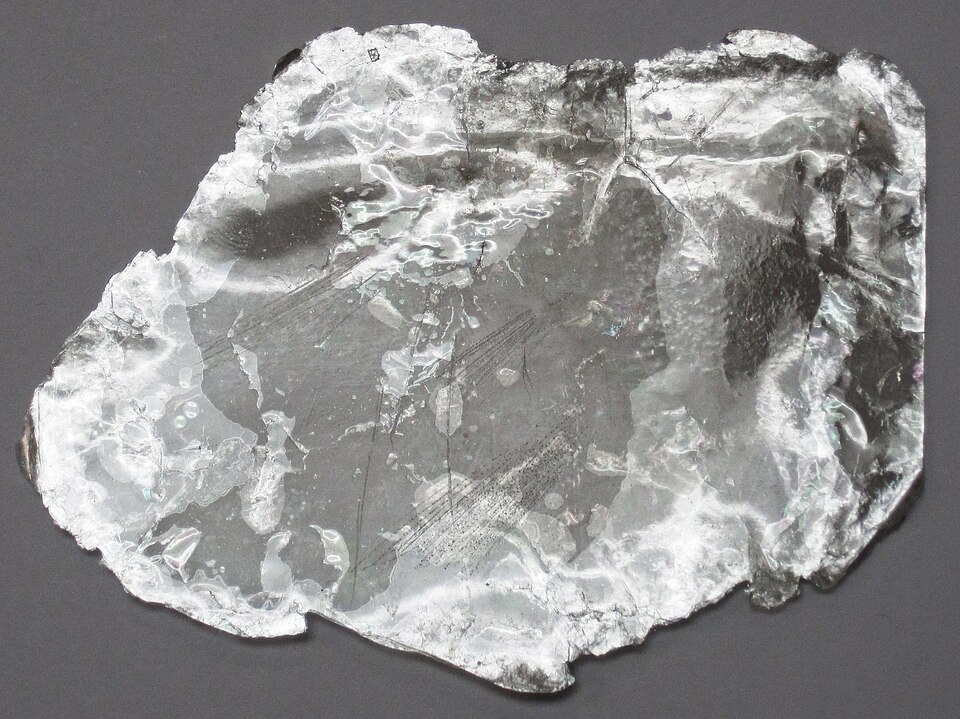
\includegraphics[height=4.2cm]{images/book1/g6-mica.jpg}
\end{minipage}\hfill
\begin{minipage}[c]{0.28\linewidth}
{\small À gauche~: un cristal de quartz, avec ses faces planes. À
droite~: une feuille de mica, un \omterm{def:g6:rocks-and-minerals:mineral}{minéral} qui se débite en paillettes très
fines. (Photos~: James St.~John, CC BY 2.0, via Wikimedia Commons.)}
% ledger: commons:jsj-rocks
\end{minipage}
\end{omfigure}

Dans le granite, les grains ont grandi serrés les uns contre les autres~:
ils n'ont donc pas de jolies formes, et ils s'emboîtent comme un puzzle.
Leur taille raconte une histoire. Le granite se forme en profondeur, là où
la \omterm{def:g3:stones-pebbles-sand:rock}{roche} fondue refroidit très lentement~: ses grains ont le temps de
devenir assez gros pour être vus à l'œil nu. La \omterm{def:g3:stones-pebbles-sand:rock}{roche} fondue qui refroidit
vite en surface, sous forme de \omterm{def:g4:volcanoes-earthquakes-first-look:eruption}{lave}, donne des \omterm{def:g3:stones-pebbles-sand:rock}{roches} aux grains trop
petits pour être vus.
% ledger: usgs:mineral-rock

\section{Les trois familles de roches}

Les géologues classent les \omterm{def:g3:stones-pebbles-sand:rock}{roches} en trois familles, non pas d'après leur
couleur, mais d'après la façon dont elles se sont formées.

\begin{definition}[Les trois familles de roches]\label{def:g6:rocks-and-minerals:rock-families}
Une \emph{roche ignée}\index{roche ignee@roche ignée} se forme quand une
\omterm{def:g3:stones-pebbles-sand:rock}{roche} fondue refroidit et devient solide~: le granite en profondeur, le
basalte à partir de la \omterm{def:g4:volcanoes-earthquakes-first-look:eruption}{lave}.
Une \emph{roche sédimentaire}\index{roche sedimentaire@roche sédimentaire}
se forme à la surface de la Terre à partir de grains de \omterm{def:g3:stones-pebbles-sand:sand}{sable} et de \omterm{def:g3:stones-pebbles-sand:sand}{boue},
ou de coquilles d'êtres vivants, déposés en couches puis durcis~: le grès,
l'argilite, le calcaire.
Une \emph{roche métamorphique}\index{roche metamorphique@roche métamorphique}
est une \omterm{def:g3:stones-pebbles-sand:rock}{roche} qui a été transformée, sans fondre, par la chaleur et la
pression en profondeur~: le marbre (issu du calcaire), l'ardoise (issue de
l'argilite).
% ledger: usgs:mineral-rock, usgs:sedimentary, usgs:metamorphic, geo:marble, geo:slate
\end{definition}

Le nom \emph{ignée} vient du mot latin qui veut dire «~feu~». Les \omterm{def:g6:rocks-and-minerals:rock-families}{roches
sédimentaires} montrent souvent des couches, posées les unes sur les
autres, comme les pages d'un livre. Les \omterm{def:g6:rocks-and-minerals:rock-families}{roches métamorphiques} sont souvent
écrasées et plissées~; certaines, comme l'ardoise, se débitent en feuilles
plates.
% ledger: usgs:mineral-rock, usgs:sedimentary, usgs:metamorphic

Beaucoup de \omterm{def:g6:rocks-and-minerals:rock-families}{roches sédimentaires} sont faites des grains que tu as triés par
taille au \cref{ch:g3:stones-pebbles-sand}~: \omterm{def:g3:stones-pebbles-sand:pebble}{galets} et \omterm{def:g3:stones-pebbles-sand:pebble}{graviers}, \omterm{def:g3:stones-pebbles-sand:sand}{sable},
\omterm{def:g3:stones-pebbles-sand:sand}{boue}. Une fois enfouis, les grains perdent leur eau et sont collés entre
eux par un ciment naturel. La taille des grains donne son nom à la \omterm{def:g3:stones-pebbles-sand:rock}{roche}.
% ledger: usgs:sedimentary, usgs:wentworth

\begin{omfigure}
\begin{tikzpicture}[
    col/.style={draw=black!60, rounded corners=2pt, minimum width=3.6cm, minimum height=1.9cm},
    lab/.style={font=\scriptsize, align=center}]
  % gravel -> conglomerate
  \node[col, fill=omLithCongl!50] (g) at (0,0) {};
  \foreach \x/\y/\r in {-1.2/0.4/0.32, -0.4/-0.3/0.4, 0.5/0.35/0.3, 1.25/-0.35/0.33, 0.2/-0.55/0.18, -1.3/-0.5/0.22}
    \fill[gray!55, draw=black!60] (\x,\y) circle (\r);
  \node[lab, above=2pt] at (g.north) {\textbf{graviers}\\ plus de 2~mm};
  \node[lab, below=3pt] (cg) at (g.south) {$\downarrow$ enfouis et cimentés\\ \textbf{conglomérat}};
    % sand -> sandstone
  \pgfmathsetseed{7}

  \node[col, fill=omLithSand!60] (s) at (4.2,0) {};
  \foreach \i in {1,...,70} \fill[brown!60!black] ({4.2+1.65*rand},{0.82*rand}) circle (0.045);
  \node[lab, above=2pt] at (s.north) {\textbf{sable}\\ de 2~mm à $\frac{1}{16}$~mm};
  \node[lab, below=3pt] at (s.south) {$\downarrow$ enfoui et cimenté\\ \textbf{grès}};
  % mud -> shale
  \node[col, fill=omLithShale!70] (m) at (8.4,0) {};
  \foreach \y in {-0.75,-0.5,...,0.8} \draw[black!35, line width=0.3pt] (6.75,\y) -- (10.05,\y);
  \node[lab, above=2pt] at (m.north) {\textbf{boue} (silt et argile)\\ moins de $\frac{1}{16}$~mm};
  \node[lab, below=3pt] at (m.south) {$\downarrow$ enfouie et tassée\\ \textbf{argilite}};
\end{tikzpicture}

{\small Trois \omterm{def:g6:rocks-and-minerals:rock-families}{roches sédimentaires} qui doivent leur nom à la taille de leurs
grains (grains très agrandis~; le \omterm{def:g3:stones-pebbles-sand:sand}{sable} est représenté à l'échelle de la
case, les \omterm{def:g3:stones-pebbles-sand:pebble}{graviers} plus gros).}
% ledger: usgs:wentworth, usgs:sedimentary
\end{omfigure}

\begin{inthefield}[Lire les pierres d'une ville]
Les villes sont des collections de \omterm{def:g3:stones-pebbles-sand:rock}{roches} en plein air. Promène-toi avec un
adulte le long de vieux murs, d'escaliers, de statues, de façades d'églises
et de pavés, et regarde de près, sans rien gratter ni rien casser. Certaines
bordures de trottoir et certaines marches sont en granite~: cherche son
quartz vitreux et son mica brillant. Beaucoup de vieux murs et de vieilles
façades sont en calcaire ou en grès~: cherche des coquilles, ou frotte du
bout du doigt une miette de grès tombée par terre pour sentir le \omterm{def:g3:stones-pebbles-sand:sand}{sable}. Les
toits peuvent être en ardoise, débitée en feuilles fines. Note dans un
carnet où se trouve chaque pierre, sa couleur, ses grains et la famille à
laquelle tu penses qu'elle appartient~; une photographie aide à comparer
ensuite avec le tableau de ce chapitre.
\end{inthefield}

\section{Le cycle des roches}

Les \omterm{def:g3:stones-pebbles-sand:rock}{roches} ne sont pas éternelles. Une \omterm{def:g1:landscapes-around-us:landform}{montagne} de granite est lentement
altérée~; ses grains sont emportés par les \omterm{def:g1:landscapes-around-us:water}{rivières} jusqu'à la \omterm{def:g2:water-on-earth:ocean}{mer} et s'y
déposent en couches~; enfouies de plus en plus profondément, les couches
durcissent en grès. Si le grès est entraîné encore plus profond, la
chaleur et la pression le transforment en \omterm{def:g6:rocks-and-minerals:rock-families}{roche métamorphique}~; plus
profond encore, il peut fondre, et la \omterm{def:g3:stones-pebbles-sand:rock}{roche} fondue, en refroidissant,
forme une nouvelle \omterm{def:g6:rocks-and-minerals:rock-families}{roche ignée}. Peu à peu, au fil de millions d'années, la
matière des \omterm{def:g3:stones-pebbles-sand:rock}{roches} tourne en rond, sans fin.
% ledger: usgs:sedimentary, usgs:metamorphic

\begin{definition}[Cycle des roches]\label{def:g6:rocks-and-minerals:rock-cycle}
Le \emph{cycle des roches}\index{cycle des roches} est le voyage sans fin
par lequel les \omterm{def:g3:stones-pebbles-sand:rock}{roches} de chaque famille sont lentement changées en \omterm{def:g3:stones-pebbles-sand:rock}{roches}
des autres familles~: par l'\omterm{def:g5:water-shapes-the-land:weathering}{altération} et l'\omterm{def:g5:water-shapes-the-land:erosion}{érosion} en surface, par
l'enfouissement et le durcissement, par la chaleur et la pression, par la
fusion et le refroidissement.
\end{definition}

\begin{omfigure}
\begin{tikzpicture}[
    fam/.style={draw, rounded corners=4pt, thick, align=center, minimum width=3.2cm,
                minimum height=1.0cm, font=\small\bfseries},
    stage/.style={draw, dashed, rounded corners=4pt, align=center, minimum width=3.0cm,
                  minimum height=0.9cm, font=\small},
    arr/.style={-{Stealth[length=2.6mm]}, thick},
    lab/.style={font=\scriptsize, align=center, fill=white, inner sep=1.5pt}]
  \node[fam, fill=omLithGranite!60] (ign) at (0,3.6) {roches ignées\\[-1pt]{\normalfont\scriptsize granite, basalte}};
  \node[stage, fill=orange!15] (grains) at (6.6,3.6) {grains de sable\\et de boue};
  \node[fam, fill=omLithSand!70] (sed) at (6.6,0) {roches sédimentaires\\[-1pt]{\normalfont\scriptsize grès, argilite, calcaire}};
  \node[fam, fill=omLithSchist!60] (met) at (0,0) {roches métamorphiques\\[-1pt]{\normalfont\scriptsize marbre, ardoise}};
  \node[stage, fill=red!12] (melt) at (-4.2,1.8) {roche fondue\\en profondeur};
  \draw[arr] (ign) -- node[lab, above] {altération\\et érosion} (grains);
  \draw[arr] (grains) -- node[lab, right] {déposés en couches,\\enfouis, durcis} (sed);
  \draw[arr] (sed) -- node[lab, below=2pt] {chaleur et pression,\\en profondeur} (met);
  \draw[arr] (met) -- node[lab, below left] {fusion} (melt);
  \draw[arr] (melt) -- node[lab, above left] {refroidissement} (ign);
  \draw[arr, black!55] (met.north east) to[bend left=12] node[lab, pos=0.45, left=4pt, text=black!60] {altération} ([xshift=-6pt]grains.south west);
  \draw[arr, black!55] (sed.north west) to[bend left=10] (grains.south west);
\end{tikzpicture}

{\small Le \omterm{def:g6:rocks-and-minerals:rock-cycle}{cycle des roches}. Chaque flèche prend de quelques milliers à
plusieurs millions d'années. Toute \omterm{def:g3:stones-pebbles-sand:rock}{roche} qui remonte à la surface peut être
altérée (flèches grises).}
% ledger: usgs:sedimentary, usgs:metamorphic, usgs:mineral-rock
\end{omfigure}

\section{Reconnaître les roches courantes}

Voici sept \omterm{def:g3:stones-pebbles-sand:rock}{roches} que l'on rencontre souvent dans les bâtiments, les
trottoirs et les \omterm{def:g1:landscapes-around-us:landscape}{paysages}.

\begin{omfigure}
\newcommand{\gsixrock}[2]{\begin{minipage}[t]{0.235\linewidth}\centering
  \includegraphics[width=\linewidth, height=0.72\linewidth, keepaspectratio=false]{images/book1/#1}\\[1pt]
  {\footnotesize #2}\end{minipage}}
\gsixrock{g6-granite.jpg}{granite}\hfill
\gsixrock{g6-basalt.jpg}{basalte}\hfill
\gsixrock{g6-sandstone.jpg}{grès}\hfill
\gsixrock{g6-limestone.jpg}{calcaire (avec des coquilles)}\par\medskip
\gsixrock{g6-shale.jpg}{argilite}\hspace{0.02\linewidth}%
\gsixrock{g6-marble.jpg}{marbre}\hspace{0.02\linewidth}%
\gsixrock{g6-slate-roof.jpg}{ardoise, sur un toit}

\medskip
{\small Sept \omterm{def:g3:stones-pebbles-sand:rock}{roches} courantes. (Photos~: James St.~John, CC BY 2.0~; toit~:
Øyvind Holmstad, CC0~; via Wikimedia Commons.)}
% ledger: commons:jsj-rocks, commons:roof-slates
\end{omfigure}

\begin{center}
\small
\begin{tabular}{>{\raggedright\arraybackslash}p{0.13\linewidth}>{\raggedright\arraybackslash}p{0.15\linewidth}>{\raggedright\arraybackslash}p{0.6\linewidth}}
\hline
\omterm{def:g3:stones-pebbles-sand:rock}{roche} & famille & ce qu'il faut observer\\
\hline
granite & ignée & de gros grains de plusieurs couleurs~: feldspath rose ou blanc, quartz gris et vitreux, mica noir et brillant\\
basalte & ignée & gris foncé à noir, grains trop petits pour être vus, souvent de petits trous ronds laissés par des bulles de gaz\\
grès & sédimentaire & des grains de \omterm{def:g3:stones-pebbles-sand:sand}{sable} que l'on sent au toucher, rugueux comme du papier de verre\\
calcaire & sédimentaire & clair, souvent avec des coquilles~; fait des bulles sous une goutte d'acide dilué\\
argilite & sédimentaire & très fine et tendre, faite de \omterm{def:g3:stones-pebbles-sand:sand}{boue} durcie (argile)~; en couches fines\\
marbre & métamorphique & blanc ou coloré, fait de cristaux brillants qui scintillent comme du sucre~; fait des bulles sous l'acide\\
ardoise & métamorphique & grise, très fine, se débite en feuilles fines, dures et plates\\
\hline
\end{tabular}
% ledger: nps:granite-minerals, geo:basalt, usgs:sedimentary, geo:limestone, geo:marble, geo:slate
\end{center}

\begin{safety}
Le test à l'acide n'est fait que par un adulte, avec des lunettes de
protection et des gants, avec un acide très dilué. Ne goûte jamais une
\omterm{def:g3:stones-pebbles-sand:rock}{roche} ni une poudre, et ne casse jamais de \omterm{def:g3:stones-pebbles-sand:rock}{roches} avec un outil~:
l'observation à la loupe en dit déjà beaucoup.
% ledger: geo:limestone
\end{safety}

Une clé de détermination est une liste de questions, chacune à deux
réponses, qui mène pas à pas au nom d'une \omterm{def:g3:stones-pebbles-sand:rock}{roche}.

\begin{omfigure}
\begin{tikzpicture}[
    q/.style={draw, rounded corners=3pt, fill=omRecall!10, align=center, text width=3.7cm,
              font=\scriptsize, inner sep=3pt},
    r/.style={draw, rounded corners=3pt, thick, fill=omLithSand!40, font=\scriptsize\bfseries,
              align=center, minimum width=1.7cm, inner sep=3pt},
    arr/.style={-{Stealth[length=2mm]}, thick}, yn/.style={font=\scriptsize\itshape, fill=white, inner sep=1pt}]
  \node[q] (q1) at (0,0) {Fait-elle des bulles sous une goutte d'acide dilué~?};
  \node[q] (q2) at (-3.4,-1.6) {Vois-tu des coquilles, ou a-t-elle un aspect terne et fin~?};
  \node[r] (lime) at (-4.8,-3.4) {calcaire};
  \node[r, align=center] (marb) at (-2.0,-3.4) {marbre\\[-1pt]{\normalfont\tiny cristaux brillants}};
  \node[q] (q3) at (3.2,-1.6) {Vois-tu des grains de plusieurs couleurs, roses, gris, noirs~?};
  \node[r] (gran) at (6.9,-1.6) {granite};
  \node[q] (q4) at (3.2,-3.2) {Sombre, grains trop petits pour être vus, petits trous ronds~?};
  \node[r] (bas) at (6.9,-3.2) {basalte};
  \node[q] (q5) at (3.2,-4.8) {Rugueuse comme du papier de verre, faite de grains de sable~?};
  \node[r] (sand) at (6.9,-4.8) {grès};
  \node[q] (q6) at (3.2,-6.4) {Dure, se débitant en feuilles fines et plates~?};
  \node[r] (slat) at (6.9,-6.4) {ardoise};
  \node[r] (shal) at (3.2,-7.8) {argilite};
  \draw[arr] (q1) -| node[yn, pos=0.25] {oui} (q2);
  \draw[arr] (q1) -| node[yn, pos=0.25] {non} (q3);
  \draw[arr] (q2.south-|lime) -- node[yn, right] {oui} (lime);
  \draw[arr] (q2.south-|marb) -- node[yn, right] {non} (marb);
  \foreach \a/\b in {q3/gran, q4/bas, q5/sand, q6/slat}{\draw[arr] (\a) -- node[yn, above] {oui} (\b);}
  \foreach \a/\b in {q3/q4, q4/q5, q5/q6, q6/shal}{\draw[arr] (\a) -- node[yn, right] {non} (\b);}
\end{tikzpicture}

{\small Une clé de détermination des sept \omterm{def:g3:stones-pebbles-sand:rock}{roches} du tableau. Commence en
haut et réponds à chaque question par oui ou par non.}
% ledger: geo:limestone, geo:marble, nps:granite-minerals, geo:basalt, usgs:sedimentary, geo:slate
\end{omfigure}

\paragraph{La dureté.} Un indice de plus aide à reconnaître un \omterm{def:g6:rocks-and-minerals:mineral}{minéral}~:
la facilité avec laquelle on peut le rayer.

\begin{definition}[Dureté et échelle de Mohs]\label{def:g6:rocks-and-minerals:hardness}
La \emph{dureté}\index{durete@dureté} d'un \omterm{def:g6:rocks-and-minerals:mineral}{minéral} est sa résistance à la
rayure~: un \omterm{def:g6:rocks-and-minerals:mineral}{minéral} raye tous ceux qui sont plus tendres que lui et il est
rayé par tous ceux qui sont plus durs. L'\emph{échelle de Mohs}\index{echelle de Mohs@échelle de Mohs}
classe la dureté de 1 à 10 à l'aide de dix \omterm{def:g6:rocks-and-minerals:mineral}{minéraux} de référence, du talc
(1), le plus tendre, au diamant (10), le plus dur.
% ledger: nps:mohs-ladder, nps:mohs-testers
\end{definition}

\begin{omfigure}
\begin{tikzpicture}[x=1cm, y=0.62cm]
  \draw[thick, black!60] (0,0.5) -- (0,10.5);
  \foreach \n/\m in {1/talc, 2/gypse, 3/calcite, 4/fluorine, 5/apatite,
                     6/feldspath (orthose), 7/quartz, 8/topaze, 9/corindon, 10/diamant}{
    \fill[omRecall!25, draw=black!50] (-0.32,\n-0.32) rectangle (0.32,\n+0.32);
    \node[font=\scriptsize\bfseries] at (0,\n) {\n};
    \node[font=\scriptsize, anchor=east] at (-0.5,\n) {\m};}
  \foreach \v/\t in {2.5/ongle, 3.5/pièce de cuivre, 5.5/verre, 6.5/clou en acier}{
    \draw[red!70!black, thick] (0.4,\v) -- (1.0,\v);
    \node[font=\scriptsize, red!70!black, anchor=west] at (1.05,\v) {\t\ (environ \v)};}
  \node[font=\scriptsize\itshape, anchor=south] at (0,10.6) {plus dur};
  \node[font=\scriptsize\itshape, anchor=north] at (0,0.4) {plus tendre};
  \node[font=\scriptsize, align=left, anchor=west, text width=6.2cm] at (4.3,5.5)
    {Un ongle raye le talc et le gypse, mais pas la calcite. Une pièce de
     cuivre raye la calcite. Le quartz raye le verre et l'acier~; aucun des
     quatre testeurs ne raye le quartz. Le mica, à 2 ou 3, se raye tout
     juste avec un ongle.};
\end{tikzpicture}

{\small L'\omterm{def:g6:rocks-and-minerals:hardness}{échelle de Mohs} (à gauche~: les dix \omterm{def:g6:rocks-and-minerals:mineral}{minéraux} de référence) et
quatre testeurs de tous les jours (à droite, en rouge).}
% ledger: nps:mohs-ladder, nps:mohs-testers, geo:mica-hardness
\end{omfigure}

\begin{method}[Le test de la rayure]\label{met:g6:rocks-and-minerals:scratch}
\begin{enumerate}
  \item Essaie de rayer le \omterm{def:g6:rocks-and-minerals:mineral}{minéral} avec ton ongle, puis avec une pièce de
        cuivre. (Le verre et l'acier ne sont utilisés que par un adulte.)
  \item Frotte la marque avec un doigt~: une vraie rayure reste, une trace
        de poudre laissée par le testeur s'efface.
  \item La \omterm{def:g6:rocks-and-minerals:hardness}{dureté} est comprise entre celle du testeur le plus dur qui ne le
        raye pas et celle du testeur le plus tendre qui le raye.
\end{enumerate}
\end{method}

\begin{example}[Quartz ou calcite~?]\label{ex:g6:rocks-and-minerals:quartz-calcite}
Deux \omterm{def:g6:rocks-and-minerals:mineral}{minéraux} blancs se ressemblent. Le premier est rayé par une pièce de
cuivre~: sa \omterm{def:g6:rocks-and-minerals:hardness}{dureté} est inférieure à 3.5~; c'est de la calcite (3). Le
second n'est pas rayé par un clou en acier et raye le verre~: sa \omterm{def:g6:rocks-and-minerals:hardness}{dureté}
est supérieure à 6.5~; parmi les \omterm{def:g6:rocks-and-minerals:mineral}{minéraux} de référence, c'est du quartz
(7).
% ledger: nps:mohs-ladder, nps:mohs-testers
\end{example}

\section{Exercices}

\begin{exercise}[$\star$]\label{exo:g6:rocks-and-minerals:1}
À quelle famille appartient chaque \omterm{def:g3:stones-pebbles-sand:rock}{roche}~: granite, grès, marbre, basalte,
calcaire, ardoise~?
\end{exercise}

\begin{exercise}[$\star$]\label{exo:g6:rocks-and-minerals:2}
Le quartz est-il un \omterm{def:g6:rocks-and-minerals:mineral}{minéral} ou une \omterm{def:g3:stones-pebbles-sand:rock}{roche}~? Et le granite~? Explique la
différence en une phrase.
\end{exercise}

\begin{exercise}[$\star$]\label{exo:g6:rocks-and-minerals:3}
Range ces \omterm{def:g6:rocks-and-minerals:mineral}{minéraux} dans l'ordre, du plus tendre au plus dur~: quartz,
talc, diamant, calcite. Lequel peut rayer tous les autres~?
\end{exercise}

\begin{exercise}[$\star$]\label{exo:g6:rocks-and-minerals:4}
Recopie et complète avec les mots \emph{refroidissement},
\emph{chaleur et pression}, \emph{\omterm{def:g5:water-shapes-the-land:weathering}{altération}}~: «~Une \omterm{def:g3:stones-pebbles-sand:rock}{roche} fondue devient
une \omterm{def:g6:rocks-and-minerals:rock-families}{roche ignée} par \ldots{} Un calcaire devient un marbre par \ldots{} Un
granite se transforme en grains de \omterm{def:g3:stones-pebbles-sand:sand}{sable} par \ldots~»
\end{exercise}

\begin{exercise}[$\star\star$]\label{exo:g6:rocks-and-minerals:5}
Utilise la clé. (a) Une \omterm{def:g3:stones-pebbles-sand:rock}{roche} ne fait pas de bulles sous l'acide~; elle est
sombre, avec des grains trop petits pour être vus et de petits trous ronds.
(b) Une \omterm{def:g3:stones-pebbles-sand:rock}{roche} fait des bulles sous l'acide et elle est faite de cristaux
brillants qui scintillent comme du sucre. (c) Une \omterm{def:g3:stones-pebbles-sand:rock}{roche} ne fait pas de
bulles~; elle est rugueuse comme du papier de verre. Nomme chaque \omterm{def:g3:stones-pebbles-sand:rock}{roche}.
\end{exercise}

\begin{exercise}[$\star\star$]\label{exo:g6:rocks-and-minerals:6}
Un \omterm{def:g6:rocks-and-minerals:mineral}{minéral} est rayé par une pièce de cuivre mais pas par un ongle. Entre
quelles deux valeurs de \omterm{def:g6:rocks-and-minerals:hardness}{dureté} se trouve-t-il~? Quel \omterm{def:g6:rocks-and-minerals:mineral}{minéral} de référence
de l'échelle de Mohs pourrait-il être~?
\end{exercise}

\begin{exercise}[$\star\star$]\label{exo:g6:rocks-and-minerals:7}
% exercise data: figdata/grade-6/granite_mosaic.py (33 / 21 / 6 grains)
Dans le dessin du granite de ce chapitre, il y a 60 grains~: 33 de
feldspath, 21 de quartz et 6 de mica. Quel pourcentage des grains est du
quartz~? Du feldspath~? Du mica~? Vérifie que les trois pourcentages font
bien 100~\% au total.
\end{exercise}

\begin{exercise}[$\star\star$]\label{exo:g6:rocks-and-minerals:8}
Le granite et le basalte sont tous deux des \omterm{def:g6:rocks-and-minerals:rock-families}{roches ignées}. Pourquoi
pouvons-nous voir à l'œil nu les grains du granite, mais pas ceux du
basalte~?
\end{exercise}

\begin{exercise}[$\star\star$]\label{exo:g6:rocks-and-minerals:9}
Le marbre est issu du calcaire. (a) À quelle famille appartient chacun
d'eux~? (b) Qu'est-il arrivé au calcaire pour qu'il se transforme en
marbre~? (c) Pourquoi tous deux font-ils des bulles sous l'acide~?
\end{exercise}

\begin{exercise}[$\star\star$]\label{exo:g6:rocks-and-minerals:10}
À l'aide de l'échelle de Mohs~: (a) le quartz peut-il rayer une bouteille
en verre~? (b) Et la fluorine~? (c) Un clou en acier peut-il rayer le
feldspath~?
\end{exercise}

\begin{exercise}[$\star\star\star$]\label{exo:g6:rocks-and-minerals:11}
Raconte le voyage d'un grain de quartz, en cinq étapes, depuis une \omterm{def:g1:landscapes-around-us:landform}{montagne}
de granite jusqu'à une \omterm{def:g6:rocks-and-minerals:rock-families}{roche métamorphique}. Nomme le phénomène à chaque
étape, et la famille de la \omterm{def:g3:stones-pebbles-sand:rock}{roche} au départ et à l'arrivée.
\end{exercise}

\begin{exercise}[$\star\star\star$]\label{exo:g6:rocks-and-minerals:12}
Un \omterm{def:g6:rocks-and-minerals:mineral}{minéral} gris et vitreux n'est pas rayé par un clou en acier, raye le
verre et est rayé par la topaze. (a) Quelle est sa \omterm{def:g6:rocks-and-minerals:hardness}{dureté} sur l'\omterm{def:g6:rocks-and-minerals:hardness}{échelle de
Mohs}~? Nomme-le. (b) Des grains de \omterm{def:g3:stones-pebbles-sand:sand}{sable} sont roulés pendant des années par
les vagues et les \omterm{def:g1:landscapes-around-us:water}{rivières}. À l'aide de sa \omterm{def:g6:rocks-and-minerals:hardness}{dureté}, explique pourquoi les
grains de ce \omterm{def:g6:rocks-and-minerals:mineral}{minéral} durent bien plus longtemps que des grains de calcite
ou de mica.
\end{exercise}

\section{Problème~: Les pierres de la place de la ville}

\begin{problem}[{Problème du week-end --- les roches d'une place de ville, le
minéral le plus dur qu'elles contiennent, et combien de familles de roches sont présentes}]
\label{pb:g6:rocks-and-minerals:1}
% ledger: nps:granite-minerals, geo:limestone, geo:slate, geo:marble, nps:mohs-ladder, nps:mohs-testers, geo:mica-hardness
Lors d'une sortie scolaire, la classe observe les pierres de la vieille
place de la ville (en observant seulement~: personne ne casse ni ne raye
les monuments). L'enseignante a apporté, de chez le tailleur de pierre,
des morceaux détachés des mêmes pierres pour les tests de \omterm{def:g6:rocks-and-minerals:hardness}{dureté}.

\smallskip
\noindent\textbf{La fontaine}~: son bassin montre de gros grains, roses,
        blancs, gris et vitreux, et noirs et brillants.
\textbf{Le pavage}~: des dalles claires où l'on voit de petites coquilles
        fossiles~; une goutte d'acide dilué, déposée par l'enseignante sur
        un morceau détaché, fait des bulles.
\textbf{Le toit de la mairie}~: des feuilles fines, plates et grises d'une
        pierre au grain très fin.
\textbf{La statue}~: une pierre blanche faite de cristaux brillants qui
        scintillent comme du sucre~; elle fait des bulles, elle aussi.

\medskip
\noindent\textbf{Partie I --- La fontaine, le pavage, le toit.}
\begin{enumerate}
  \item Nomme la \omterm{def:g3:stones-pebbles-sand:rock}{roche} de la fontaine et sa famille. Nomme ses trois
        \omterm{def:g6:rocks-and-minerals:mineral}{minéraux}.
  \item Nomme la \omterm{def:g3:stones-pebbles-sand:rock}{roche} du pavage et sa famille. Qu'étaient les coquilles
        avant de se trouver dans la pierre~?
  \item Nomme la \omterm{def:g3:stones-pebbles-sand:rock}{roche} du toit et sa famille. À partir de quelle \omterm{def:g3:stones-pebbles-sand:rock}{roche}
        s'est-elle formée~?
  \item Nomme la \omterm{def:g3:stones-pebbles-sand:rock}{roche} de la statue et sa famille. À partir de quelle \omterm{def:g3:stones-pebbles-sand:rock}{roche}
        s'est-elle formée~?
\end{enumerate}

\medskip
\noindent\textbf{Partie II --- Un test de dureté.}
\begin{enumerate}[resume]
  \item L'enseignante essaie de rayer un grain gris et vitreux de la
        fontaine avec un clou en acier~: aucune rayure. Le grain raye le
        verre. Quel est ce \omterm{def:g6:rocks-and-minerals:mineral}{minéral}, et quelle est sa \omterm{def:g6:rocks-and-minerals:hardness}{dureté}~?
  \item Les grains roses sont rayés par le clou en acier mais pas par le
        verre. Entre quelles deux valeurs se trouve leur \omterm{def:g6:rocks-and-minerals:hardness}{dureté}~? De quel
        \omterm{def:g6:rocks-and-minerals:mineral}{minéral} de l'échelle de Mohs s'agit-il~?
  \item Les paillettes noires se rayent tout juste avec un ongle. Quel
        \omterm{def:g6:rocks-and-minerals:mineral}{minéral} est-ce~?
  \item Une pièce de cuivre peut-elle rayer le pavage~? Explique à l'aide
        de la \omterm{def:g6:rocks-and-minerals:hardness}{dureté} de la calcite.
\end{enumerate}

\medskip
\noindent\textbf{Partie III --- Le cycle des roches.}
\begin{enumerate}[resume]
  \item Après des siècles de \omterm{def:g4:clouds-rain-snow:precipitation}{pluie}, la statue a perdu ses détails fins.
        Quel phénomène du \omterm{def:g6:rocks-and-minerals:rock-cycle}{cycle des roches} est à l'œuvre~?
  \item Le granite de la fontaine vient d'une \omterm{def:g1:landscapes-around-us:landform}{montagne}. Au fil de millions
        d'années, que pourraient devenir les grains de quartz de cette
        \omterm{def:g1:landscapes-around-us:landform}{montagne}, et dans quelle \omterm{def:g3:stones-pebbles-sand:rock}{roche} pourraient-ils finir~?
  \item Combien des trois familles de \omterm{def:g3:stones-pebbles-sand:rock}{roches} sont présentes sur la
        place~? Nomme la ou les \omterm{def:g3:stones-pebbles-sand:rock}{roches} de chacune.
  \item Quelle est la \omterm{def:g6:rocks-and-minerals:hardness}{dureté} de Mohs du \omterm{def:g6:rocks-and-minerals:mineral}{minéral} le plus dur que l'on trouve
        dans les pierres de la place~?
\end{enumerate}
\end{problem}
